% !TEX encoding = UTF-8 Unicode

\documentclass[a4paper]{article}

\usepackage{array}

\usepackage{color}
\usepackage{url}
%\usepackage[T2A]{fontenc} % enable Cyrillic fonts
\usepackage[utf8]{inputenc} % make weird characters work
\usepackage{graphicx}

\usepackage[english,serbian]{babel}
%\usepackage[english,serbianc]{babel} %ukljuciti babel sa ovim opcijama, umesto gornjim, ukoliko se koristi cirilica

\usepackage[unicode]{hyperref}
\hypersetup{colorlinks,citecolor=green,filecolor=green,linkcolor=blue,urlcolor=blue}

%\newtheorem{primer}{Пример}[section] %ćirilični primer
%\newtheorem{primer}{Primer}[section]


\usepackage{adjustbox}

%\definecolor{mygreen}{rgb}{0,0.6,0}
%\definecolor{mygray}{rgb}{0.5,0.5,0.5}
%\definecolor{mymauve}{rgb}{0.58,0,0.82}
\usepackage[section]{placeins}

\FloatBarrier

\usepackage{listings}
\usepackage{xcolor}
\definecolor{verde}{rgb}{0.25,0.5,0.35}
\definecolor{jpurple}{rgb}{0.5,0,0.35}
\definecolor{darkgreen}{rgb}{0.0, 0.2, 0.13}
\definecolor{white}{rgb}{1, 1, 1}
%\usepackage{listings}

\newcommand{\CSharp}{
	\lstset{
		language=Java,
		basicstyle=\ttfamily\footnotesize,
		keywordstyle=\color{jpurple}\bfseries,
		stringstyle=\color{red},
		commentstyle=\color{verde},
		morecomment=[s][\color{blue}]{/**}{*/},
		extendedchars=true,
		showspaces=false,
		showstringspaces=false,
		numbers=left,
		numberstyle=\tiny,
		breaklines=true,
		backgroundcolor=\color{white},
		breakautoindent=true,
		captionpos=b,
		xleftmargin=0pt,
		tabsize=2
}}



\lstset{ 
	backgroundcolor=\color{white},   % choose the background color; you must add \usepackage{color} or \usepackage{xcolor}; should come as last argument
	basicstyle=\tiny\ttfamily,        % the size of the fonts that are used for the code
	breakatwhitespace=false,         % sets if automatic breaks should only happen at whitespace
	breaklines=true,                 % sets automatic line breaking
	captionpos=b,                    % sets the caption-position to bottom
	commentstyle=\color{mygreen},    % comment style
	deletekeywords={...},            % if you want to delete keywords from the given language
	escapeinside={\%*}{*)},          % if you want to add LaTeX within your code
	extendedchars=true,              % lets you use non-ASCII characters; for 8-bits encodings only, does not work with UTF-8
	firstnumber=1000,                % start line enumeration with line 1000
	frame=single,	                   % adds a frame around the code
	keepspaces=true,                 % keeps spaces in text, useful for keeping indentation of code (possibly needs columns=flexible)
	keywordstyle=\color{blue},       % keyword style
	language=Python,                 % the language of the code
	morekeywords={*,...},            % if you want to add more keywords to the set
	numbers=left,                    % where to put the line-numbers; possible values are (none, left, right)
	numbersep=5pt,                   % how far the line-numbers are from the code
	numberstyle=\tiny\color{mygray}, % the style that is used for the line-numbers
	rulecolor=\color{black},         % if not set, the frame-color may be changed on line-breaks within not-black text (e.g. comments (green here))
	showspaces=false,                % show spaces everywhere adding particular underscores; it overrides 'showstringspaces'
	showstringspaces=false,          % underline spaces within strings only
	showtabs=false,                  % show tabs within strings adding particular underscores
	stepnumber=2,                    % the step between two line-numbers. If it's 1, each line will be numbered
	stringstyle=\color{mymauve},     % string literal style
	tabsize=1,	                   % sets default tabsize to 2 spaces
	title=\lstname                   % show the filename of files included with \lstinputlisting; also try caption instead of title
}

\begin{document}
	
	\title{C\# AST fix\\ \small{Seminarski rad u okviru kursa\\Verifikacija softvera\\ Matematički fakultet}}
	
	\author{Ana Petrović, 1073/2020, pana.petrovic@gmail.com, \\ Aleksandra Dotlić, 1077/2020, alexandra.nerandzic@gmail.com, \\ Branko Đaković, 1083/2019, brankodjakovic08@gmail.com, \\ Jovana Pejkić, 1089/2020, jovanadpejkic@gmail.com}
	
	\maketitle
	
	\abstract{
		
		Tokom razvoja softvera neretko dolazi do propusta u arhitekturi, pisanju koda, testiranju, dokumentovanju i ostalim fazama razvoja. Upravo zbog toga treba voditi računa o svim fazama i posebno se posvetiti svakoj od njih. Da bi kod bio kvalitetniji, greške i propuste treba uočiti na vreme i ispraviti. Od velikog značaja za kvalitet softvera jeste analiza izvornog koda i zamena nepodobnih sintaksnih formi odgovarajućim, čime se ovaj rad bavi, a uz pomoć čega se može postići značajna memorijska i vremenska ušteda, kao i razni drugi benefiti.
		
		\tableofcontents
		
		\newpage
		
		\section{Opis problema}
		\label{sec:opis_problema}
		
		Zadatak koji je rešavan u okviru ovog projekta je analiza koda u jeziku \textit{C\#}, detektovanje i popravka neispravnih ili nedovoljno dobrih sintaksnih konstrukata. Nakon konstantovanja problema, korisniku neće biti (samo) prijavljeno upozorenje i sugestija kako se kod može popraviti, već će se vršiti uklanjanje ili zamena nepoželjnih konstrukata onima koji su poželjniji. Uz sve ovo, funkcionalnost koda ne sme biti promenjena.
		
		Cilj ovog rada je kreiranje kvalitetnijeg koda, bez suvišnih delova, kompleksnih fragmenata i nečitljive sintakse. To je način da se izvorni kod "očisti" i tako smanji mogućnost za pojavu grešaka.
		
		U nastavku, u okviru ove sekcije je detaljnije opisano \textbf{refaktorisanje} - proces koji predstavlja navedene transformacije (podsekcija \ref{subsec:refaktorisanje}). Dalje, u podsekciji \ref{subsec:koriscene_tehnologije} su opisane tehnologije koje su korišćene.
		
		
		\subsection{Refaktorisanje}
		\label{subsec:refaktorisanje}
		
		Refaktorisanje je proces (postupak) kojim se postojeći kod menja tako da bude čitljiviji i manje kompleksan. Ključna stvar je da izmene koda ne utiču na funkcionalnost samog koda. Cilj je poboljšanje dizajna, strukture i/ili implementacije softvera, uz očuvanje njegove funkcionalnosti. Ovo može poboljšati održavanje izvornog koda i stvoriti jednostavniju, čistiju i izražajniju unutrašnju arhitekturu. Osim toga, proces refaktorisanja može uticati i na poboljšanje performansi.
		
		
		% Manual refactoring are often error-prone and timeconsuming [2]. For instance, renaming a method requires checking that the method’s new name is not yet in use as well as updating all invocations. Besides being obviously time-consuming this operation is also error-prone because polymorphism may cause a forgotten update to compile correctly but change the software’s behaviour inadvertently. This requires the maintainer to manually locate the changed functionality and update the omitted invocation. As a result, these refactoring are often not performed and the software’s structure deteriorates as a result of functional changes. 
		
		%\begin{lstlisting}[caption={Primer ubacivanja koda u tekst},frame=single, label=simple]
		%# This program ...
		%print 'Please supply integer arguments'
		%\end{lstlisting}
		
		\subsection{Korišćene tehnologije}
		\label{subsec:koriscene_tehnologije}
		
		Sve transformacije su pisane u jeziku \textit{C\#} uz korišćenje .NET platforme za kompajliranje (eng. \textit{.NET Compiler Platform}) pod nazivom \textbf{Rozlin}
		(eng. \textit{Roslyn}), opisane u podsekciji \ref{subsubsec:rozlin}. Za testiranje rezultata ovih transformacija pisani su testovi koji predstavljaju jednostavne programe, takođe pisane u jeziku \textit{C\#}. Projekat je rađen u okruženju \textit{Visual Studio}.
		
		\subsubsection{Rozlin}
		\label{subsubsec:rozlin}
		
		Rozlin je platforma koju čini skup kompajlera otvorenog koda (eng. \textit{open-source compilers}) i interfejsa za analizu koda (eng. \textit{code analysis APIs}) za \textit{C\#} i \textit{Visual Basic} (\textit{VB.NET}) Majkrosoftove jezike. Rozlin je dizajniran tako da olakša razvoj alata za analizu izvornog koda. Ova .NET platforma ima tri vrste APIja: \textit{feature APIs}, \textit{work-space APIs} i \textit{compiler APIs}, koji su detaljnije opisani u tabeli \ref{tab:tabela}.
		
		\begin{center}
			\label{tab:tabela} %TODO ne prikazuje 1 kada se referise vec 1.2.1
			\begin{tabular}{ | m{3cm} | m{6cm} | } 
				\hline
				\textbf{\textit{Feature APIs}} & dozvoljavaju \textit{source code tool} programerima da refaktorišu i isprave kod  \\ 
				\hline
				\textbf{\textit{Work-space APIs}} & dozvoljavaju korišćenje plugina za, na primer, pronalaženje referenci promenljive ili oblikovanja koda (eng. \textit{code formatting})  \\ 
				\hline
				\textbf{\textit{Compiler APIs}} & dopuštaju još elegantniju analizu izvornog koda, izlaganjem (odnosno upućivanjem) direktnih poziva za izvođenje sintaksnog stabla i analizom toka vezivanja (eng. \textit{binding flow analysis})  \\ 
				\hline
			\end{tabular}
			%\caption{Table caption} %TODO caption ne radi
		\end{center}
		
		
		
		\section{Opis arhitekture sistema}
		\label{sec:opis_arhitekture_sistema}
		
		%TODO
		U ovoj sekciji bice opisano ......... \textbf{TODO}
		
		\hfill
		
		%TODO
		- \textbf{TODO} Opis osnovnih modula implementacije
		%TODO
		- \textbf{TODO} Reprezentacija sistema na visokom nivou
		%TODO
		- \textbf{TODO} Način na koji je program razložen na komponente
		
		\hfill
		
		Na slici \ref{fig:CSharpSyntaxRewriter} je prikazana hijerarhija klasa koje su korišćene za izvršavanje transformacija. Ono što je za sve implementirane klase zajedničko, jeste da sve one nasleđuju klasu \textit{CSharpSyntaxRewriter} i implementiraju metode u skladu sa transformacijom koju vrše.
		
		\begin{figure}[!htb]
			\begin{center}
				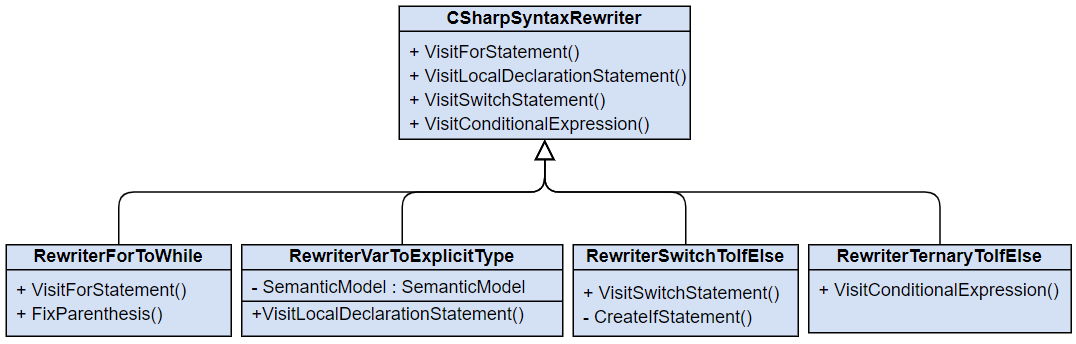
\includegraphics[scale=0.5]{images/CSharpSyntaxRewriter.png}
			\end{center}
			\caption{Nasleđivanje klase \textit{CSharpSyntaxRewriter}}
			\label{fig:CSharpSyntaxRewriter}
		\end{figure}
		
		Na slici \ref{fig:IChecker} su prikazani različiti čekeri. Ove klase naseđuju \textit{IChecker} klasu i implementiraju metod \textit{Check}.
		
		\begin{figure}[!htb]
			\begin{center}
				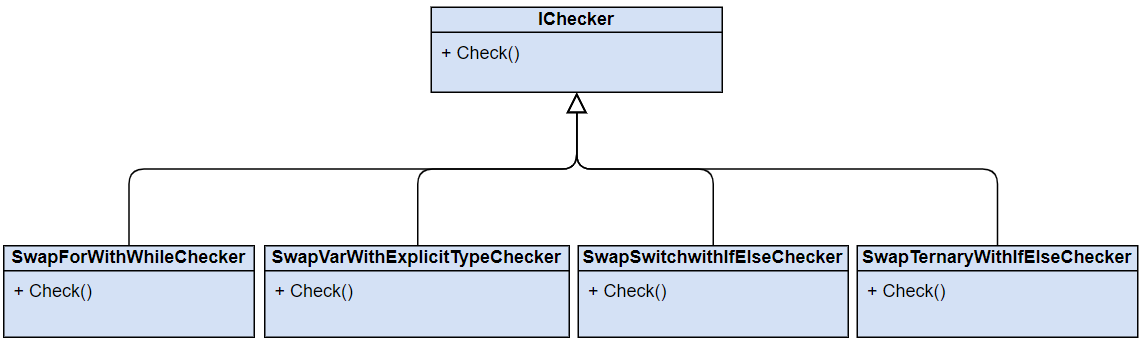
\includegraphics[scale=0.5]{images/IChecker.png}
			\end{center}
			\caption{Nasleđivanje klase \textit{IChecker}}
			\label{fig:IChecker}
		\end{figure}
		
		
		\section{Opis rešenja problema}
		\label{sec:opis_resenja_problema}
		
		Osnovna ideja je da se u \textit{.cs} fajlu, čija se putanja dobija od strane korisnika, izvrši pronalaženje i zamena nepodobnih programskih konstrukata odgovarajućim (bez promene semantike koda) i tako izmenjen kod upiše u \textit{.cs} fajl, čiju putanju, opet, zadaje korisnik. Stoga, rad programa je zasnovan na analizi izvornog koda i adekvatnim transformacijama. Preciznije, najpre se određeni konstrukti pretražuju u kodu a zatim i zamenjuju onima koji su poželjniji. Primer transformacije može biti zamena \textit{for} petlje u \textit{while} petlju, zamena ključne reči \textit{var} u eksplicitni tip promenljive i slično. Namera je da se korisniku ukaže na nepravilne, nečitljive konstrukte, ali i da se prikaže bolje rešenje za konkretan slučaj. Ideja je da ove transformacije vrše različiti "prepisivači" (eng. \textit{Rewriters}) - klase u kojima se redefinišu metode nadklase \textit{CSharpSyntaxRewriter}. U projektu su implementirani sledeći "prepisivači":
		\begin{itemize}
			\item RewriterForToWhile - zamenjuje for petlju u while
			\item RewriterVarToExplicitType - zamenjuje ključnu rec var sa eksplicitnim tipom
			\item RewriterSwitchToIfElse - zamenjuje switch naredbu if-else naredbom
			\item RewriterRemoveEmptyStatements - eliminiše prazne naredbe
		\end{itemize}
		
		Sam program se sastoji od nekoliko čekera (eng. \textit{Chekers}) i "prepisivača", gde čekeri pozivaju metod \textit{Visit} nad instancom neke od \textit{Rewriter} klasa. Klase \textit{SwapForWithWhileChecker} i \textit{RewriterForToWhile} su opisane u podsekciji \ref{subsec:for}, klase \textit{SwapVarWithExplicitTypeChecker} i \textit{RewriterVarToExplicitType} u podsekciji \ref{subsec:var}, klase \textit{SwapSwitchWithIfElseChecker} i \textit{RewriterSwitchToIfElse} u podsekciji \ref{subsec:switch}, a klase \textit{RemoveEmptyStatementsChecker} i \textit{RewriterRemoveEmptyStatements} u podsekciji \ref{subsec:prazne}. Kod je organizovan u nabrojanim klasama kako bi bio čitljiviji i tako da svaka klasa predstavlja jednu celinu.
		
		Za kreiranje i transformaciju stabla Rozlin nudi dve mogućnosti: \textit{Factory} metodi su najbolji izbor kada je potrebno zameniti specifičan čvor, ili ukoliko postoji specifična lokacija na kojoj je potrebno dodati nov čvor. \textit{Rewriters} su najbolja opcija kada treba skenirati ceo projekat kako bi u kodu bili pronađeni (prepoznati) šabloni (eng. \textit{code patterns}) koje je potrebno zameniti.
		
		U nastavku ove sekcije je prikazan osnovni algoritam, tako što je detaljno opisana svaka od implementiranih klasa. U podsekciji \ref{subsec:for} je opisana zamena \textit{for} petlje u \textit{while} petlju, u podsekciji \ref{subsec:var} je opisana zamena ključne reči \textit{var} u eksplicitni tip promenljive, zatim je u podsekciji \ref{subsec:switch} opisana zamena naredbe  \textit{switch} u \textit{if-else} naredbu, i na kraju u podsekciji \ref{subsec:prazne} je opisana eliminacija praznih naredbi.
		
		%Glavni .cs fajl Progeram.cs sadrzi main funkciju u kojoj se od korisnika zahteva unos putanje do .cs fajla koji treba da bude transformisan (izmenjen), a zatim se kreira tree, model i odgovarajuci ceker nad kojim se poziva metod Check koji kao argumente prima tree i model. Na kraju se vrsi parsiranje teksta... prevodi se u string.
		
		\subsection{Zamena for petlje u while petlju}
		\label{subsec:for}
		
		Iako se i \textit{for} i \textit{while} petljom postižu slični rezultati, odluka o tome koja će biti iskorišćena u mnogim slučajevima zavisi od prioriteta samog programera. Ipak, demonstracije radi, u ovoj sekciji će biti prikazana zamena \textit{for} petlje \textit{while} petljom. Ukoliko se u datom \textit{.cs} fajlu naiđe na konstrukciju oblika kao u kodu \ref{lst:forloop}, to će biti zamenjeno \textit{while} petljom kao što je prikazano u kodu \ref{lst:whileloop}.
		
		
		\CSharp
		\begin{lstlisting}[caption={For petlja}, label=lst:forloop]
		for (int i = 0; i < 5; i++) {
		...
		}
		\end{lstlisting}
		
		
		\CSharp
		\begin{lstlisting}[caption={While petlja}, label=lst:whileloop]
		int i = 0;
		
		while (i < 5) {
		...
		i++;
		}
		\end{lstlisting}
		
		
		Kao i za svaku transformaciju, i ovde se koriste klase \textit{Checker} i \textit{Rewriter}. Klasa \textit{SwapForWithWhileChecker} je prikazana na slici \ref{fig:SwapForWithWhileChecker}. Ova klasa nasleđuje klasu \textit{IChecker} i u njoj je implementiran metod \textit{Check} koji kao argumente prima sintaksno stablo i semantički model. Unutar ovog metoda kreira se instanca klase \textit{RewriterForToWhile} nad kojom se poziva metod \textit{Visit} kome se prosleđuje koren datog stabla. Ovaj metod radi ???????? i kao povratnu vrednost ovaj metod vraća ?????? %TODO . 
		Dodatno, na početku svakog čekera, navodi se opcija za argument komandne linije koju je potrebno uključiti za konkretnu transformaciju. U ovom slučaju to je "\textit{-forToWhile}".
		
		\begin{figure}[!h]
			\begin{center}
				
				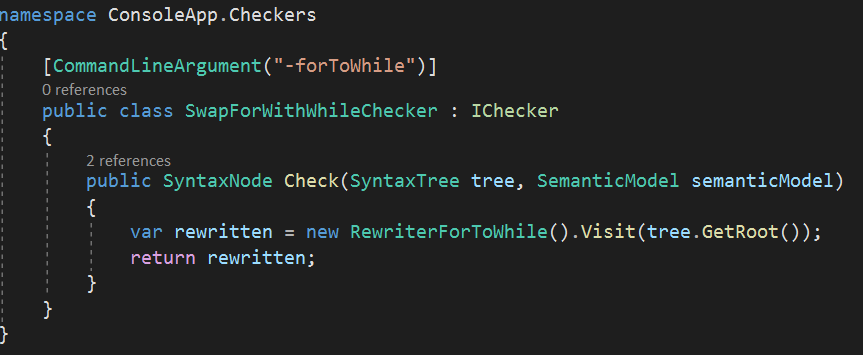
\includegraphics[scale=0.65]{images/SwapForWithWhileChecker2.png}
			\end{center}
			\caption{Klasa \textit{SwapForWithWhileChecker}}
			\label{fig:SwapForWithWhileChecker}
		\end{figure}
		
		
		Dalje, klasa \textit{RewriterForToWhile} (prikazana na slici \ref{fig:RewriterForToWhile}) nasleđuje klasu \textit{CSharpSyntaxRewriter} i redefiniše metod \textit{VisitForStatement}. Ovaj metod kao argument prima čvor i, krenuvši od njega, posećuje svaku \textit{for} naredbu. Kada naiđe na takvu naredbu, proverava da li u njoj postoji deklaracija (na primer \textit{int i=0}) i, ukoliko postoji, ona biva sačuvana u promenljivu \textit{declarationNode} kako bi kasnije bila postavljena iznad \textit{while} petlje. Samo telo petlje se nalazi unutar \textit{syntaxNode.Statement}. Na osnovu ovoga, može se napraviti novi čvor koji predstavlja \textit{while} petlju. Najpre se proverava da li je for petlja imala neki uslov i, ukoliko jeste, onda se on postavlja za uslov \textit{while} petlje, a ukoliko nije, onda se za uslov \textit{while} petlje postavlja \textit{true}. Zatim se parsira telo \textit{for} petlje u \textit{while} (dodaje se inkrementiranje i slično) i postavljaju se \textit{;} tamo gde je to potrebno. Na kraju je napravljen novi čvor koji se sastoji od pomenute deklaracije promenjive i \textit{while} petlje - to je 'spojeno' i vraćeno kao jedan čvor. Implementirana je i pomoćna funkcija \textit{FixParenthesis} koja 'popravlja' zagrade pre kreiranja novog čvora.
		
		\FloatBarrier
		\begin{figure}[!htb]
			\begin{center}
				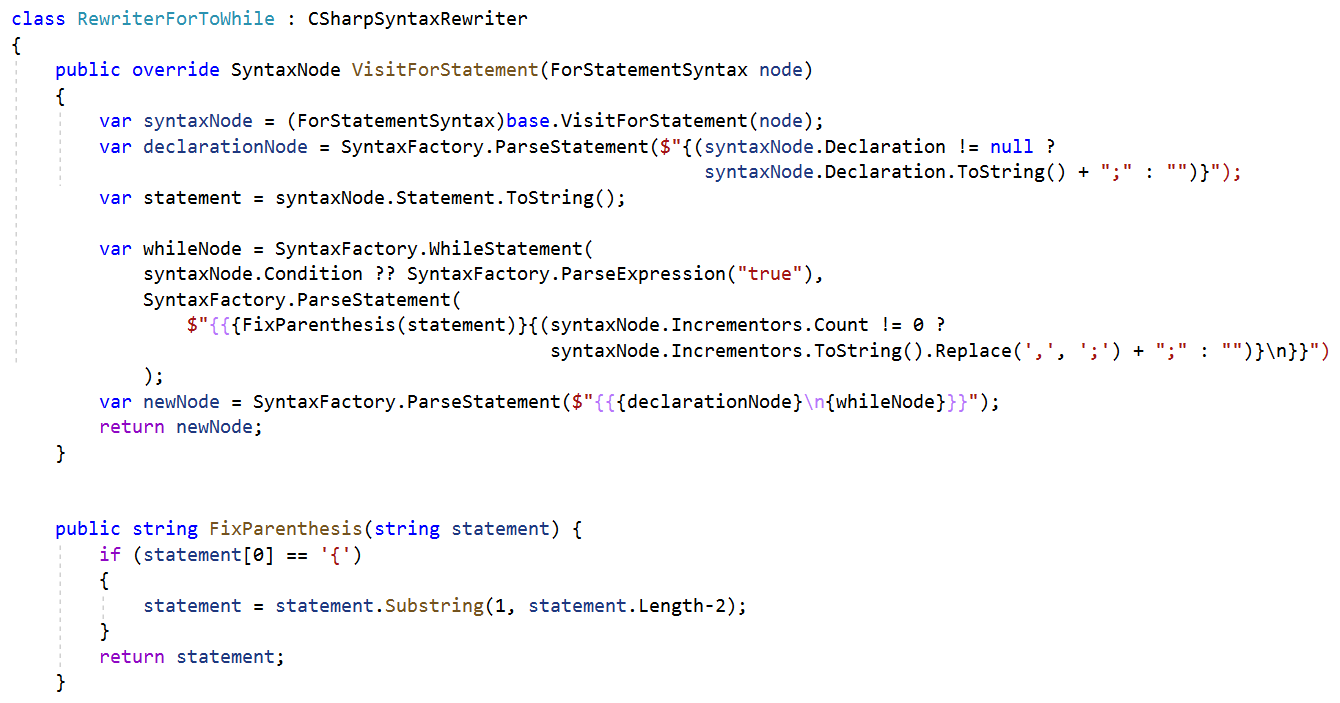
\includegraphics[scale=0.44]{images/RewriterForToWhile.png}
			\end{center}
			\caption{Klasa \textit{RewriterForToWhile}}
			\label{fig:RewriterForToWhile}
		\end{figure}
		\FloatBarrier
		
		\subsection{Zamena ključne reči var u eksplicitni tip}
		\label{subsec:var}
		Pri lokalnoj deklaraciji promenljivih u jeziku C\#, promenljivoj se može dodeliti implicitni tip navođenjem ključne reči \textit{var}.  U nekim slučajevima, takav kod je preporučljivo refaktorisati promenom deklaracije takvih promenljivih u eksplicitan tip - npr. kada nije neophodno inicijalizovati promenljivu u samoj deklaraciji, ili jednostavno da bi se dobio čitljiviji kod. U nastavku (kod \ref{lst:var} i \ref{lst:explicit}) su prikazani oblici sintaksnog konstrukta pre i nakon zamene. 
		\CSharp
		\begin{lstlisting}[caption={Var promenljiva}, label=lst:var]
		var i = 5;
		if(i<10)
		var a = i + 1.3;
		\end{lstlisting}
		
		\begin{lstlisting}[caption={Eksplicitan tip}, label=lst:explicit]
		int i = 5;
		if(i<10)
		double a = i + 1.3;
		\end{lstlisting}
		
		\par Slično kao u prethodnom primeru, postoji klasa koja implementira čeker - \textit{SwapVarWithExplicitTypeChecker}, i klasa koja implementira metod koji posećuje čvorove - \textit{RewriterVarToExplicitType} (Slika \ref{fig:RewriterVarToType}). U ovoj transformaciji, posećuju se čvorovi koji su tipa \textit{LocalDeclarationStatement}, odnosno deklaracija promenljive. Kako bi se dobila informacija o tipu čvora, kod je neophodno analizirati na semantičkom nivou, pa je potrebno uključiti i semantički model. Metod \textit{VisitLocalDeclarationStatement} najpre iz semantičkog modela  pokupi tip implicitne naredbe. Sa dobijenim tipom i ostatkom naredbe koji ostaje isti kao i ranije kreira se nova \textit{LocalDeclarationStatement}, pritom zadržavajući formatiranje koje je korišćeno. Na kraju, vratća se kreirana deklaracija.
		
		\FloatBarrier
		\begin{figure}[!htb]
			\begin{center}
				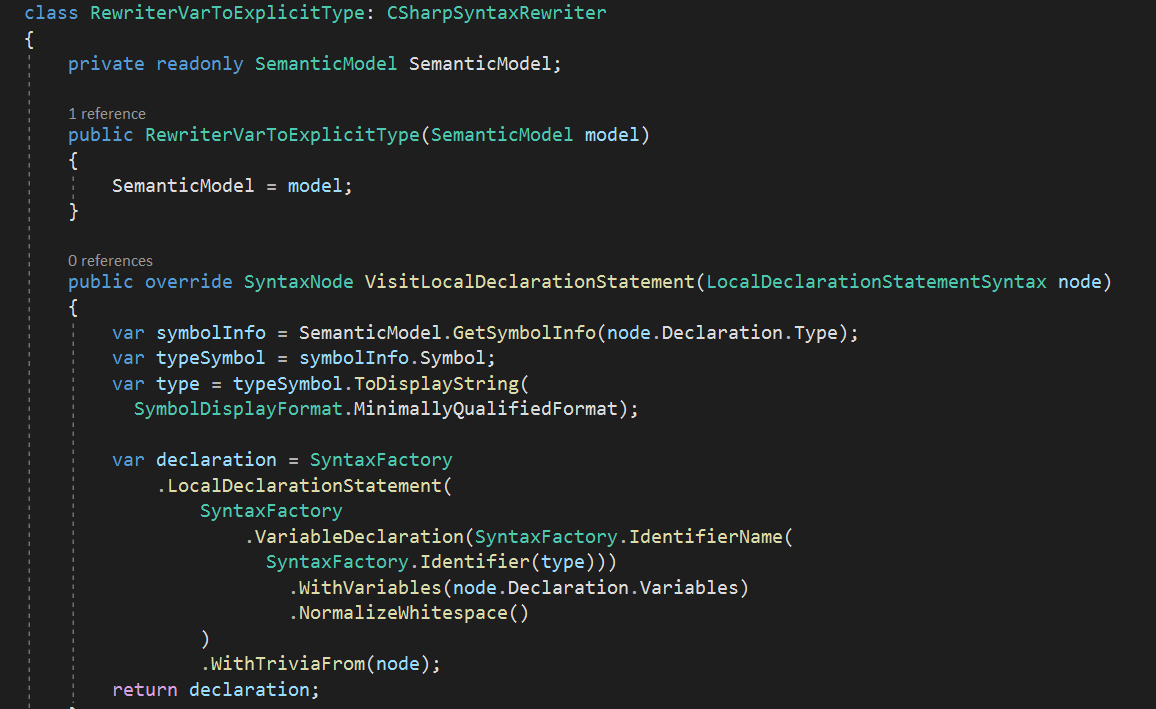
\includegraphics[scale=0.5]{images/RewriterVarToType.png}
			\end{center}
			\caption{Klasa \textit{RewriterVarToExplicitType}}
			\label{fig:RewriterVarToType}
		\end{figure}
		\FloatBarrier
		
		\subsection{Zamena switch naredbe u if-else}
		\label{subsec:switch}
		
		
		Naredbe \textit{switch} i \textit{if-else} imaju sličnu ulogu, ali je u nekim situacijama ispravnije iskoristiti jednu odnosno drugu. Na primer, ukoliko je potrebno ispitati samo jedan uslov (i u skladu sa njegovom vrednošću izvršiti odgovarajuće naredbe), preporučuje se korišćenje \textit{if-else} naredbe. Ukoliko se u kodu naiđe na konstrukte poput prikazanog u kodu \ref{lst:switch}, ova transformacija to konvertuje u oblik prikazan u kodu \ref{lst:ifelse}.
		
		
		\CSharp
		\begin{lstlisting}[caption={Switch naredba}, label=lst:switch]
		int k = 2;
		
		switch (k) {
		
		case 1:
		...
		break;
		
		case 2:
		...
		break;
		
		default:
		break;
		}
		\end{lstlisting}
		
		
		\CSharp
		\begin{lstlisting}[caption={If-else naredba}, label=lst:ifelse]
		int k = 2;
		
		if (k == 1) {
		...
		}
		else if (k == 2) {
		...
		}
		else {
		...
		}
		\end{lstlisting}
		
		
		Slično kao u prethodnim podsekcijama, ovde se najpre metodom \textit{VisitSwitchStatement} obilaze sve \textit{switch} naredbe, gde se za svaku izdvaja izraz (eng. \textit{expression}) koji figuriše u \textit{switch} naredbi, kao i obeležja (eng. \textit{labels}) i naredbe (eng. \textit{statements}) koje su različite od \textit{break} naredbe. Nakon toga, kreira se novi čvor čija se vrednost postavlja na \textit{null}. Ukoliko unutar \textit{switch} naredbe postoji samo jedno obeležje i to obeležje je \textit{default}, onda se kreira \textit{if} naredba sa uslovom \textit{true} i to postaje vrednost novog čvora.
		%TODO SyntaxFactory.Block(SyntaxFactory.ParseStatement(statements.ElementAt(0).Aggregate("", (x, y) => x.ToString() + " " + y.ToString())))).ToString());
		Inače, ukoliko postoji više od jednog obeležja, poziva se privatna funkcija \textit{CreateIfStatement()} kojoj se prosleđuju izdvojeni izraz, obeležja i naredbe. Opisani metod \textit{VisitSwitchStatement()} je dat na slici \ref{fig:RewriterSwitchToIf_part1}.
		
		
		\begin{figure}[!htb]
			\begin{center}
				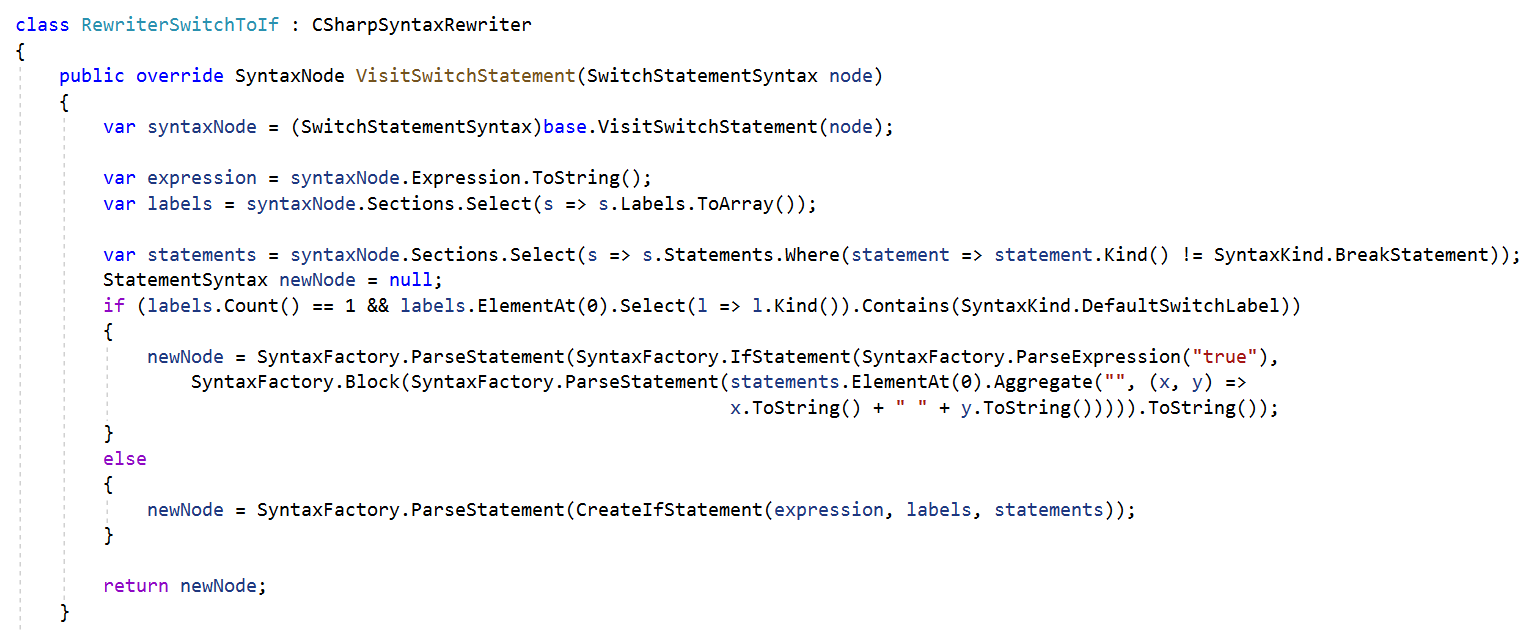
\includegraphics[scale=0.44]{images/RewriterSwitchToIf_part1.png}
			\end{center}
			\caption{Klasa \textit{RewriterSwitchToIf}, metod \textit{VisitSwitchStatement()}}
			\label{fig:RewriterSwitchToIf_part1}
		\end{figure}
		
		\begin{figure}[!htb]
			\begin{center}
				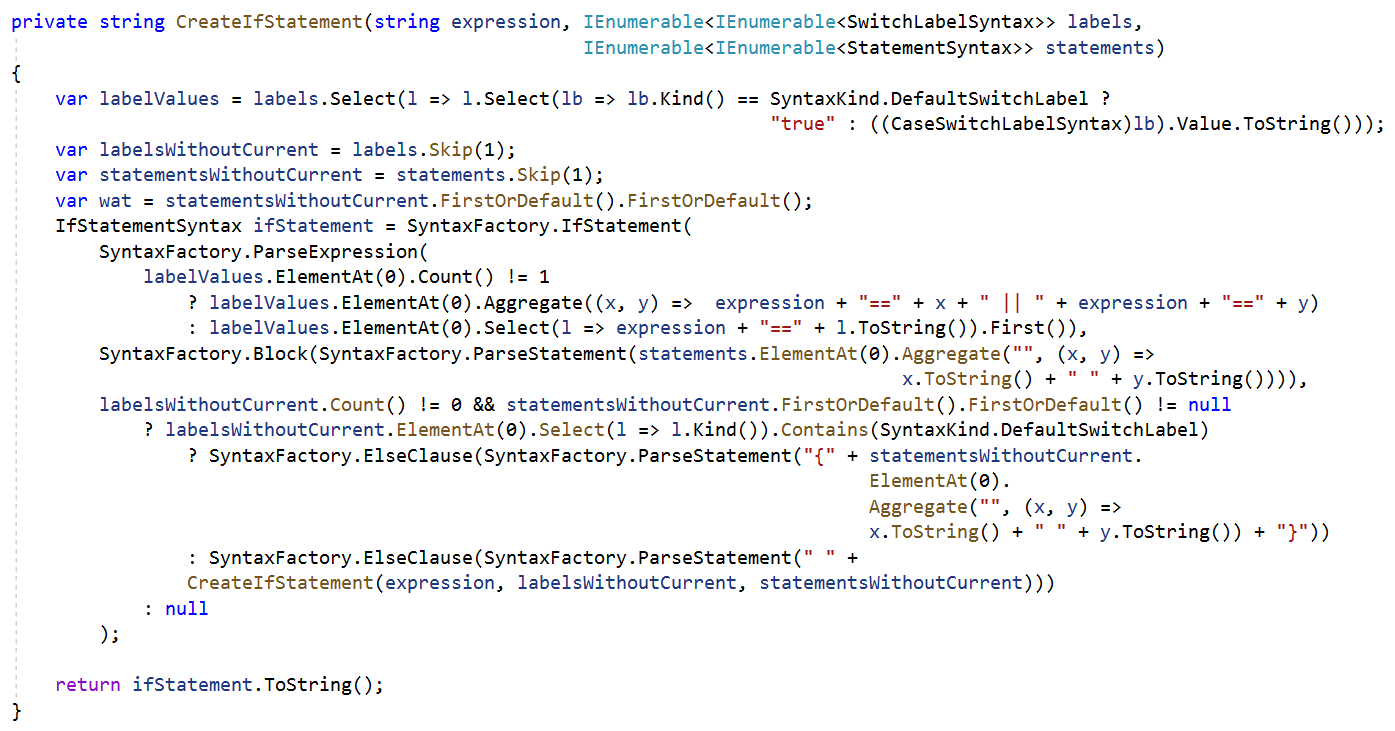
\includegraphics[scale=0.44]{images/RewriterSwitchToIf_part2.png}
			\end{center}
			\caption{Klasa \textit{RewriterSwitchToIf}, funkcija \textit{CreateIfStatement()}}
			\label{fig:RewriterSwitchToIf_part2}
		\end{figure}
		
		\subsection{Uklanjanje praznih naredbi}
		\label{subsec:prazne}
		Poslednji primer transformacije jeste ukljanjanje praznih naredbi. Prazna naredba, tj. tačka-zarez ( \textbf{;}), obično nastaje greškom, na primer kada se ostavi da bi se kasnije zamenila konkretnom naredbom, ali se to ne desi, ili greškom u kucanju (npr. ;;). Ponekad, programeri koriste praznu naredbu kao telo petlje. To nije dobra praksa, te se preporučuje izbegavanje ovakvog koda. U kodovima \ref{lst:empty} i \ref{lst:noempty} dat je primer ovakvih konstrukata i kako oni treba da izgledaju nakon tranformacije. Kad god se u kodu naiđe na praznu naredbu upotrebljenu u kontekstu u kom nije neophodna, ista se jednostavno eliminiše. 
		
		
		\begin{lstlisting}[caption={Prazna naredba}, label=lst:empty]
		void DoSomething()
		{
		; 
		}
		
		void DoSomethingElse()
		{
		Console.WriteLine("Hello, world!");; 
		
		for (int i = 0; i < 3; Console.WriteLine(i), i++); 
		}
		\end{lstlisting}
		
		
		\begin{lstlisting}[caption={Uklonjena prazna naredba}, label=lst:noempty]
		void DoSomething()
		{
		}
		
		void DoSomethingElse()
		{
		Console.WriteLine("Hello, world!");
		
		for (int i = 0; i < 3; Console.WriteLine(i), i++)
		{
		}
		}
		\end{lstlisting}
		
		
		\par Klase \textit{RemoveEmptyStatementsChecker} i \textit{RewriterRemoveEmptyStatements} implementirane su na sličan način kao i u svim prethodnim primerima. Na slici \ref{fig:RemoveEmptyRewriter} može se videti implementacija prepisivača. Metod \textit{VisitEmptyStatement} obilazi sve čvorove u stablu koji predstavljajju prazne naredbe. Vrši se provera vrste roditelja čvora, tj. provera da li se naredba nalazi unutar petlje, \textit{if} ili \textit{else} naredbe. Ako je to slučaj, vraća prazan blok (otvorena i zatvorena vitičasta zagrada \{ \}). Inače, jednostavno vrati \textit{null} - uklanja se ; . 
		
		\begin{figure}[!htb]
			\begin{center}
				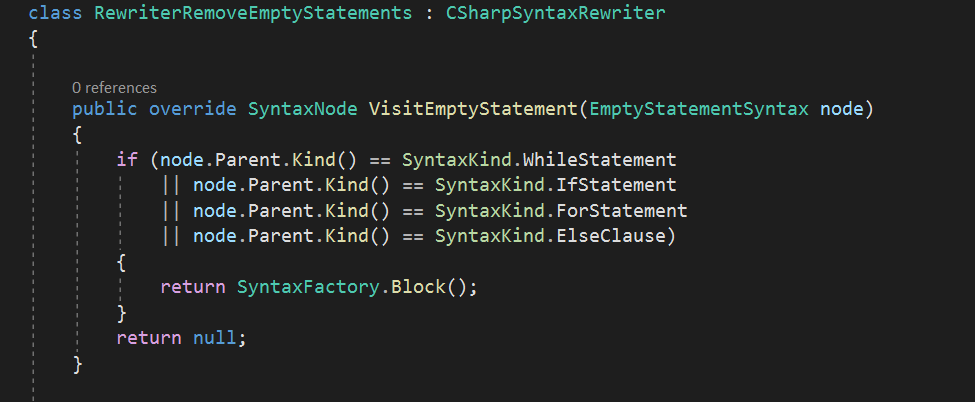
\includegraphics[scale=0.7]{images/RewriterEmpty.png}
			\end{center}
			\caption{Klasa \textit{RewriterRemoveEmptyStatements}}
			\label{fig:RemoveEmptyRewriter}
		\end{figure}
		
	\end{document}
